\documentclass[letterpaper]{article}
\usepackage{fullpage}
\usepackage[table]{xcolor}
\usepackage{tabularx}
\usepackage{graphicx}
\usepackage{amsmath}
\usepackage{hyperref}
\usepackage{listings}
\lstset{language=python, tabsize=4}

\title{Deep Learning Approach to Link Weight Prediction}

\begin{document}
\maketitle


\section{Experiments}
We evaluate Model R experimentally
and the results show that 
Model R can achieve much lower prediction error than the baseline models \cite{aicher2014learning}.

\subsection{Datasets}
The experiments use 4 datasets summarized in \autoref{tab:datasets}.
\begin{table}[!htb]
	\centering
	\caption{The datasets used in experiments.}
	\begin{tabularx}{\textwidth}{|c|c|X|c|X|}  \hline \rowcolor{blue!50}
		Dataset & Node count & Node type & Link count & Link weight type \\ \hline
		Airport\cite{colizza2007reaction} & 500 & busiest airports in US & 5960 & number of passengers traveling from one airport to the other\\ \hline
		Collaboration\cite{pan2012world} & 226 & nations on Earth & 20616 & number of academic papers written by authors from the two connected nations \\ \hline
		Congress\cite{porter2005network} & 163  & 102nd US Congress committees & 26569 & interlock value of shared members from the two committees \\ \hline
		Forum\cite{opsahl2009clustering}  & 1899 & users of a student social network at UC Irvine & 20291 & number of messages sent from one student to the other \\ \hline
	\end{tabularx}
	\label{tab:datasets}
\end{table}

\subsection{Experiment process}
We do the identical experiment for each dataset.
All the weights are normalized to ranger [-1, 1] after applying a logarithm function.
Each experiment consists of 25 independent trials.
In each trial, we split the dataset randomly into 3 subsets:
\begin{itemize}
	\item 70\% into training set
	\item 10\% into validation set
	\item 20\% into testing set
\end{itemize}
We use MSE (mean squared error) as the prediction accuracy metric of a trial.
For each experiment, we report the mean and standard deviation of the 25 MSE's.
The pseudo code of the experiment process is as follows:

\begin{lstlisting}
	def main():
		for dataset in [Airport, Collaboration, Congress, Forum]:
			(MSE_mean, MSE_standard_deviation) = do_experiment(dataset)
	def do_experiment(dataset):
		MSEs = list()
		for trial in range(25):
			testing_error = append(evaluate_model_on(dataset))
			MSEs.append(testing_error)
		return (MSEs.mean(), MSEs.standard_deviation())
	def evaluate_model_on(dataset):
		(trainning_set, validation_set, testing_set) = split(dataset)
		while validation_error decreases:
			training_error = estimator.learn(training_set)
			validation_error = estimator.predict(validation_set)
		testing_error = estimator.predict(testing_set)
		return testing_error
\end{lstlisting}

\subsection{Experiment results}
In our experiments,
Model R's prediction error is lower than every other model on every dataset,
shown in \autoref{fig:errors}.
\begin{figure}[!htb]
	\centering
	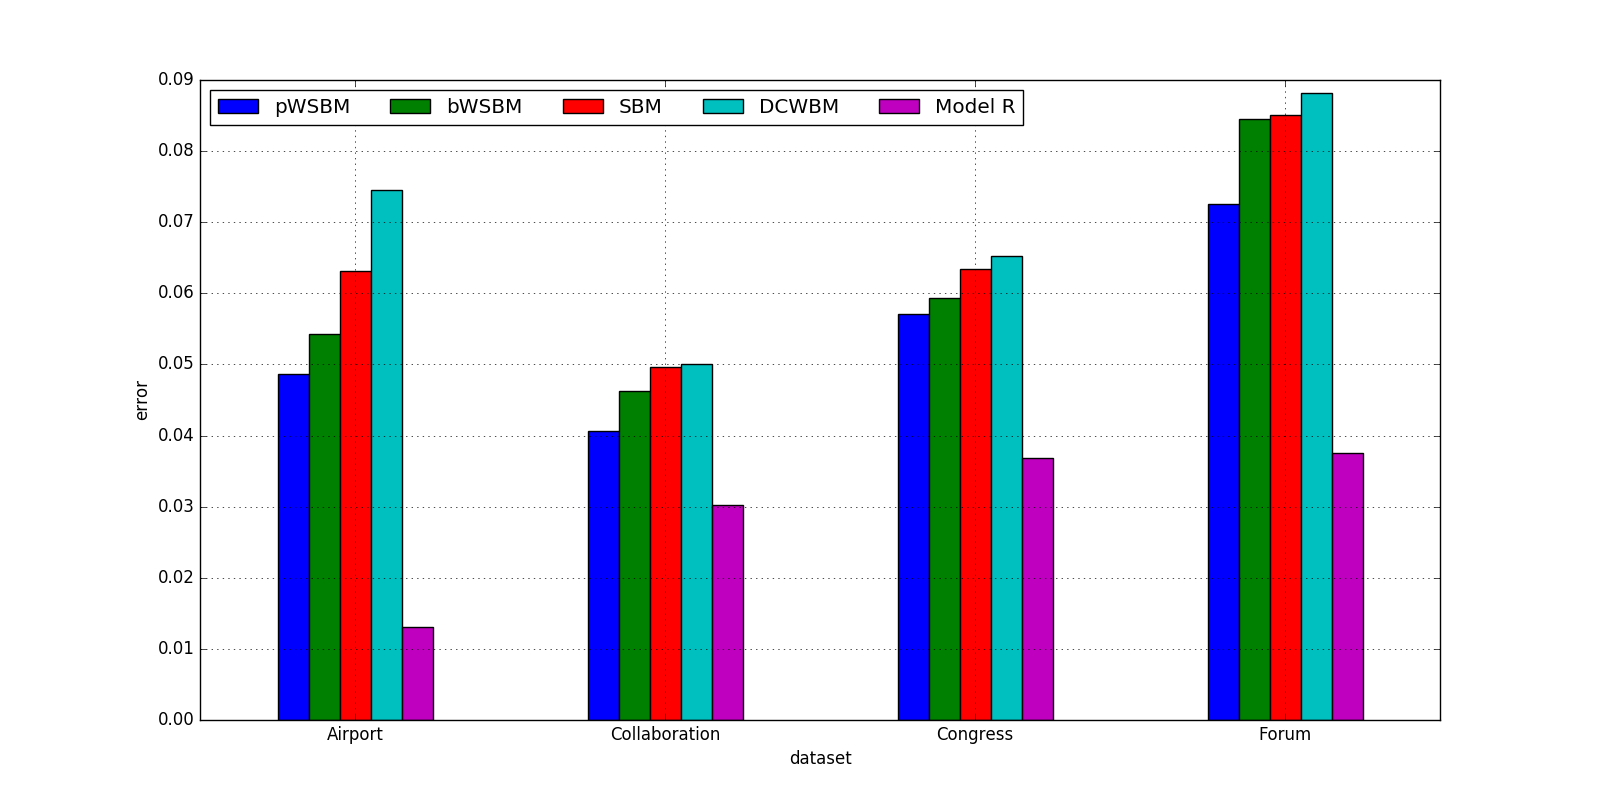
\includegraphics[width=\textwidth]{link-weight-errors}
	\caption[content...]{
		The MSE's of 6 models on 4 datasets:
		Model R has lower MSE than every other model on every dataset.
	}
	\label{fig:errors}
\end{figure}
Now we compare Model R with only best baseline model - pWSBM.
We calculate the error reduction from this best baseline model to Model R as:
\begin{align*}
	Reduction = \frac{BaselineError - ModelRError}{BaselineError}
\end{align*}
The reduction in prediction error is significant:
ranging from 25\% on Collaboration dataset to 73\% on Airport dataset,
shown in \autoref{tab:errors}.
\begin{table}[!htb]
	\centering
	\caption{
		The MSE's of 6 models on 4 datasets:
		Model R has lower error than every other model on every dataset,
		reducing error by 25\% to 73\% from the best baseline model - pWSBM.
		The number in every parenthesis is the standard deviation of MSE in 25 trials in the last digit of MSE.
	}
	\begin{tabularx}{\textwidth}{|X|c|c|c|c|c|c|c|} \hline \rowcolor{blue!50}
		Dataset & pWSBM & bWSBM & SBM & DCWBM & DCBM & Model R & Reduction \\ \hline
		Airport & 0.0486(6) & 0.0543(5) & 0.0632(8) & 0.0746(9) & 0.0918(8) & 0.013(1) & 73\% \\ \hline
		Collaboration & 0.0407(1) & 0.0462(1) & 0.0497(3) & 0.0500(2) & 0.0849(3) & 0.030(1) & 25\% \\ \hline
		Congress & 0.0571(4) & 0.0594(4) & 0.0634(6) & 0.0653(4) & 0.1050(6) & 0.036(3) & 35\% \\ \hline
		Forum & 0.0726(3) & 0.0845(3) & 0.0851(4) & 0.0882(4) & 0.0882(4) & 0.037(1) & 48\% \\ \hline
	\end{tabularx}
	\label{tab:errors}
\end{table}

\subsection{Computing resources}
We ran our experiments on a Lenovo ThinkCentre M83 machine with the following specifications:
\begin{itemize}
	\item Python implementation: CPython 3.5
	\item Operating system: Ubuntu 16.10 64-bit
	\item Memory: 16 GB
	\item Processor: Intel Core i7-4770 CPU @ 3.40GHz $ \times $ 8
\end{itemize}
The program - coded in Python - uses all 8 threads of the processor.
Each experiment takes about one hour to finish,
depending on the dataset and parameters in the learning algorithm.

\bibliographystyle{plain}
\bibliography{references}
\end{document}
